% ============================================================
% 培优专题3 — 函数与动点综合
% 编译命令：xelatex -interaction=nonstopmode 培优专题3_函数与动点综合.tex
% ============================================================
\documentclass[12pt, a4paper]{ctexart}
\usepackage[margin=2.2cm]{geometry}
\usepackage{amsmath, amssymb}
\usepackage{enumitem}
\usepackage{tcolorbox}
\usepackage{booktabs}
\usepackage{array}
\usepackage{fancyhdr}
\usepackage{xcolor}
\usepackage{tikz}
\usepackage{hyperref}
\usepackage{graphicx}
\usepackage{multirow}
\usepackage{pgfplots}
\pgfplotsset{compat=1.18}

% 颜色定义
\definecolor{mainblue}{RGB}{41, 98, 168}
\definecolor{lightblue}{RGB}{230, 240, 255}
\definecolor{tipgreen}{RGB}{34, 139, 87}
\definecolor{lightgreen}{RGB}{235, 250, 240}
\definecolor{warnred}{RGB}{200, 50, 50}
\definecolor{lightred}{RGB}{255, 240, 240}
\definecolor{examorange}{RGB}{210, 120, 20}
\definecolor{lightorange}{RGB}{255, 248, 235}
\definecolor{apppurple}{RGB}{120, 60, 170}
\definecolor{lightpurple}{RGB}{245, 238, 255}

% 页眉页脚
\pagestyle{fancy}
\fancyhf{}
\fancyhead[L]{\small\textcolor{mainblue}{\textbf{初中数学培优 · 函数与动点}}}
\fancyhead[R]{\small\textcolor{mainblue}{培优专题3}}
\fancyfoot[C]{\small —\ \thepage\ —}
\renewcommand{\headrulewidth}{0.6pt}
\renewcommand{\headrule}{\hbox to\headwidth{\color{mainblue}\leaders\hrule height \headrulewidth\hfill}}
\renewcommand{\footrulewidth}{0pt}

% tcolorbox 样式
\newtcolorbox{knowledgebox}[1][]{%
  colback=lightblue, colframe=mainblue,
  fonttitle=\bfseries\large, title=#1,
  arc=3mm, boxrule=0.8pt,
  left=8pt, right=8pt, top=6pt, bottom=6pt
}

\newtcolorbox{tipbox}[1][]{%
  colback=lightgreen, colframe=tipgreen,
  fonttitle=\bfseries, title=#1,
  arc=2mm, boxrule=0.6pt,
  left=6pt, right=6pt, top=4pt, bottom=4pt
}

\newtcolorbox{warnbox}[1][]{%
  colback=lightred, colframe=warnred,
  fonttitle=\bfseries, title=#1,
  arc=2mm, boxrule=0.6pt,
  left=6pt, right=6pt, top=4pt, bottom=4pt
}

\newtcolorbox{examplebox}[1][]{%
  colback=lightorange, colframe=examorange,
  fonttitle=\bfseries, title=#1,
  arc=3mm, boxrule=0.8pt,
  left=8pt, right=8pt, top=6pt, bottom=6pt
}

\newtcolorbox{appbox}[1][]{%
  colback=lightpurple, colframe=apppurple,
  fonttitle=\bfseries, title=#1,
  arc=3mm, boxrule=0.8pt,
  left=8pt, right=8pt, top=6pt, bottom=6pt
}

\setCJKmainfont{Hiragino Sans GB}
\setCJKsansfont{Heiti SC}

% 填空命令
\newcommand{\blank}[1]{\underline{\hspace{#1}}}

\begin{document}

% ============ 标题页 ============
\begin{center}
{\Huge\bfseries\textcolor{mainblue}{培优专题3\quad 函数与动点综合}}\\[12pt]
{\Large\textcolor{gray}{讲\quad 义}}\\[8pt]
\rule{0.6\textwidth}{1pt}\\[8pt]
{\normalsize 适用：初中数学培优\quad |\quad 课时：6--8课时}
\end{center}
\vspace{10pt}

% ============ 知识框架 ============
\begin{knowledgebox}[知识框架]
本专题综合一次函数、反比例函数、二次函数与动点问题，重点训练：
\begin{enumerate}[label=\textcolor{mainblue}{\arabic*.}]
  \item 动点在坐标轴或线段上运动时，面积、线段长度与时间的函数关系；
  \item 一次函数与几何图形的综合（面积、存在性）；
  \item 反比例函数中 $k$ 的几何意义及面积问题；
  \item 二次函数的三种表达式及图象特征（衔接九年级）；
  \item 将军饮马模型与坐标系中的最短路径；
  \item 动点背景下的存在性问题（等腰三角形、直角三角形、平行四边形、相似三角形）。
\end{enumerate}
\end{knowledgebox}

\vspace{6pt}

% ============================================================
\section*{\textcolor{mainblue}{一、一次函数与动点}}
% ============================================================

\subsection*{1.1\quad 动点在坐标轴上运动}

\begin{knowledgebox}[核心思路]
动点在坐标轴上匀速运动 $\Rightarrow$ 用时间 $t$ 表示动点坐标 $\Rightarrow$ 用坐标表示相关线段长度 $\Rightarrow$ 建立面积（或距离）关于 $t$ 的函数关系。

\medskip
\textbf{关键步骤：}
\begin{enumerate}[label=(\arabic*)]
  \item 确定动点的起点、终点、速度；
  \item 写出 $t$ 时刻动点的坐标（注意分段：动点到达端点前后）；
  \item 用割补法或底高公式表示面积；
  \item 根据动点位置变化的临界点，分段写出函数表达式。
\end{enumerate}
\end{knowledgebox}

\begin{warnbox}[易错提醒]
动点运动到端点后可能停止或折返，需要讨论 $t$ 的取值范围，面积函数往往是\textbf{分段函数}。
\end{warnbox}

% ---------- 例题 1 ----------
\begin{examplebox}[【例1】矩形中动点与面积]
如图，矩形 $OABC$ 中，$O$ 为原点，$A(0,4)$，$C(6,0)$。点 $P$ 从 $O$ 出发沿 $OC$ 以每秒1个单位的速度向 $C$ 运动，点 $Q$ 从 $C$ 出发沿 $CB$ 以每秒1个单位的速度向 $B$ 运动，两点同时出发。设运动时间为 $t$ 秒（$0\le t\le 6$），求 $\triangle OPQ$ 的面积 $S$ 关于 $t$ 的函数关系式。

\begin{center}
\begin{tikzpicture}
  \draw[thick] (0,0) rectangle (6,4);
  \node[left] at (0,2) {$O$};
  \node[left] at (0,4) {$A$};
  \node[right] at (6,4) {$B$};
  \node[right] at (6,0) {$C$};
  \draw[->,thick,mainblue] (0,0) -- (6.5,0) node[right]{$x$};
  \draw[->,thick,mainblue] (0,0) -- (0,4.5) node[above]{$y$};
  \fill[red] (3,0) circle(2pt) node[below]{$P$};
  \fill[red] (6,2) circle(2pt) node[right]{$Q$};
  \draw[thick,examorange] (0,0) -- (3,0) -- (6,2) -- cycle;
  \node[below] at (3,-0.5) {\small $t$ 时刻};
\end{tikzpicture}
\end{center}

\textbf{解：}运动时间为 $t$ 秒时，
\[P(t,\,0),\quad Q(6,\,t).\]
$\triangle OPQ$ 以 $OP$ 为底，$Q$ 到 $x$ 轴的距离为高：
\[\text{底 } OP = t,\quad \text{高 } h = t.\]
由三角形面积公式：
\[\boxed{S = \frac{1}{2}\cdot t\cdot t = \frac{t^2}{2},\quad 0\le t\le 6.}\]
\end{examplebox}

% ---------- 例题 2 ----------
\begin{examplebox}[【例2】动点在坐标轴上——分段面积函数]
如图，在平面直角坐标系中，$A(0,6)$，$B(8,0)$，$P$ 从 $A$ 出发沿 $y$ 轴负方向以每秒2个单位运动，$Q$ 从 $O$ 出发沿 $x$ 轴正方向以每秒1个单位运动，两点同时出发。设运动时间为 $t$ 秒，求四边形 $ABQP$ 的面积 $S$ 关于 $t$ 的函数关系式。

\begin{center}
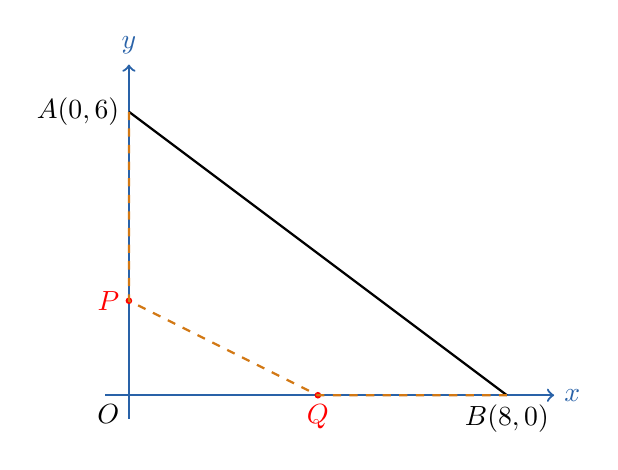
\begin{tikzpicture}[scale=0.6]
  \draw[->,thick,mainblue] (-0.5,0) -- (9,0) node[right]{$x$};
  \draw[->,thick,mainblue] (0,-0.5) -- (0,7) node[above]{$y$};
  \draw[thick] (0,6) -- (8,0);
  \node[left] at (0,6) {$A(0,6)$};
  \node[below] at (8,0) {$B(8,0)$};
  \node[below left] at (0,0) {$O$};
  \fill[red] (0,2) circle(2pt) node[left]{$P$};
  \fill[red] (4,0) circle(2pt) node[below]{$Q$};
  \draw[thick,examorange,dashed] (0,6) -- (0,2) -- (4,0) -- (8,0);
\end{tikzpicture}
\end{center}

\textbf{解：}运动 $t$ 秒时，$P(0,\,6-2t)$，$Q(t,\,0)$。

运动持续到 $P$ 到达 $O$（$t=3$）或 $Q$ 到达 $B$（$t=8$），故分段讨论。

\textbf{（i）当 $0\le t\le 3$ 时：}

$P$ 在 $O$ 上方，四边形 $ABQP$ 可以用 $\triangle AOB$ 减去 $\triangle OPQ$：
\[S_{\triangle AOB}=\frac{1}{2}\times 8\times 6=24,\]
\[S_{\triangle OPQ}=\frac{1}{2}\cdot t\cdot(6-2t)=3t-t^2.\]
\[\boxed{S=24-(3t-t^2)=t^2-3t+24,\quad 0\le t\le 3.}\]

\textbf{（ii）当 $3<t\le 8$ 时：}

$P$ 在 $O$ 下方（$P$ 到达 $O$ 后停止或继续运动，此处假设 $P$ 在 $t>3$ 时停在 $O$），$Q(t,0)$。

此时四边形退化为 $\triangle ABQ$：
\[\boxed{S=\frac{1}{2}\cdot(8-t)\cdot 6=24-3t,\quad 3<t\le 8.}\]
\end{examplebox}

% ---------- 例题 3 ----------
\begin{examplebox}[【例3】正方形中双动点]
如图，正方形 $ABCD$ 边长为 $4$，$A$ 为原点，$B(4,0)$，$D(0,4)$。点 $P$ 从 $A$ 出发沿 $AB$ 以每秒1个单位向 $B$ 运动，点 $Q$ 从 $B$ 出发沿 $BC$ 以每秒1个单位向 $C$ 运动，两点同时出发。设运动时间为 $t$ 秒。

（1）求 $\triangle DPQ$ 的面积 $S$ 与 $t$ 的关系式；

（2）当 $t$ 为何值时，$\triangle DPQ$ 是等腰三角形？

\begin{center}
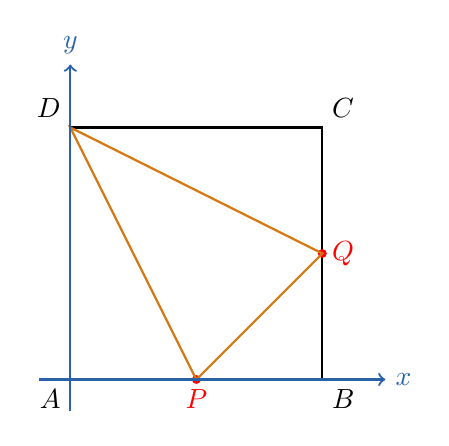
\begin{tikzpicture}[scale=0.8]
  \draw[thick] (0,0) rectangle (4,4);
  \node[below left] at (0,0) {$A$};
  \node[below right] at (4,0) {$B$};
  \node[above right] at (4,4) {$C$};
  \node[above left] at (0,4) {$D$};
  \fill[red] (2,0) circle(2pt) node[below]{$P$};
  \fill[red] (4,2) circle(2pt) node[right]{$Q$};
  \draw[thick,examorange] (0,4) -- (2,0) -- (4,2) -- cycle;
  \draw[->,thick,mainblue] (-0.5,0) -- (5,0) node[right]{$x$};
  \draw[->,thick,mainblue] (0,-0.5) -- (0,5) node[above]{$y$};
\end{tikzpicture}
\end{center}

\textbf{解：}

$P(t,0)$，$Q(4,t)$，$D(0,4)$（$0\le t\le 4$）。

\textbf{（1）}$S_{\triangle DPQ}$：用正方形面积减去三个直角三角形面积。
\[S_{ABCD}=16.\]
\[S_{\triangle ADP}=\frac{1}{2}\cdot t\cdot 4=2t,\quad
S_{\triangle PBQ}=\frac{1}{2}\cdot(4-t)\cdot t,\quad
S_{\triangle DCQ}=\frac{1}{2}\cdot 4\cdot(4-t)=2(4-t).\]
\begin{align*}
S &= 16-2t-\frac{t(4-t)}{2}-2(4-t)\\
  &= 16-2t-2t+\frac{t^2}{2}-8+2t\\
  &= \frac{t^2}{2}-2t+8.
\end{align*}
\[\boxed{S=\frac{t^2}{2}-2t+8=\frac{1}{2}(t-2)^2+6,\quad 0\le t\le 4.}\]
当 $t=2$ 时，$S$ 取最小值 $6$。

\textbf{（2）}计算各边长的平方：
\[DP^2=t^2+16,\quad DQ^2=16+(4-t)^2=t^2-8t+32,\quad PQ^2=(4-t)^2+t^2=2t^2-8t+16.\]

\textbf{情况一：}$DP=DQ$，即 $t^2+16=t^2-8t+32$，解得 $t=2$。

\textbf{情况二：}$DP=PQ$，即 $t^2+16=2t^2-8t+16$，得 $t^2-8t=0$，解得 $t=0$（舍去）或 $t=8$（舍去，超出范围）。

\textbf{情况三：}$DQ=PQ$，即 $t^2-8t+32=2t^2-8t+16$，得 $t^2=16$，解得 $t=4$。

\[\boxed{t=2 \text{ 或 } t=4.}\]
\end{examplebox}

\begin{tipbox}[方法总结：动点问题三步法]
\begin{enumerate}[label=\textbf{(\arabic*)}]
  \item \textbf{设}：设运动时间为 $t$，写出动点坐标；
  \item \textbf{表}：用 $t$ 表示相关线段长度、面积等几何量；
  \item \textbf{求}：根据条件列方程或函数关系，注意 $t$ 的取值范围，必要时分段讨论。
\end{enumerate}
\end{tipbox}

% ============================================================
\section*{\textcolor{mainblue}{二、一次函数与几何综合}}
% ============================================================

\subsection*{2.1\quad 一次函数图象与坐标轴围成的三角形面积}

\begin{knowledgebox}[基本结论]
一次函数 $y=kx+b$（$k\ne 0$）与 $x$ 轴交于 $\left(-\dfrac{b}{k},\,0\right)$，与 $y$ 轴交于 $(0,\,b)$。

与坐标轴围成的三角形面积为：
\[S = \frac{1}{2}\cdot\left|-\frac{b}{k}\right|\cdot|b| = \frac{b^2}{2|k|}.\]
\end{knowledgebox}

\subsection*{2.2\quad 两直线交点与围成图形面积}

\begin{knowledgebox}[求交点]
两直线 $y=k_1x+b_1$ 与 $y=k_2x+b_2$ 的交点坐标由方程组
\[k_1x+b_1=k_2x+b_2 \implies x=\frac{b_2-b_1}{k_1-k_2},\quad y=\frac{k_1 b_2-k_2 b_1}{k_1-k_2}.\]
求围成图形面积时，常将图形分割为以坐标轴上的线段为底的三角形。
\end{knowledgebox}

\subsection*{2.3\quad 一次函数与等腰三角形/直角三角形存在性}

\begin{knowledgebox}[存在性问题的处理方法]
\begin{enumerate}[label=(\arabic*)]
  \item 设出动点坐标（通常在已知直线上，用一个参数表示）；
  \item 根据等腰或直角条件列出方程；
  \item 分类讨论所有可能的情况；
  \item 检验解是否在有效范围内。
\end{enumerate}
\end{knowledgebox}

% ---------- 例题 4 ----------
\begin{examplebox}[【例4】两直线交点与三角形面积]
已知直线 $l_1:\,y=-x+4$ 与 $l_2:\,y=\dfrac{1}{2}x+1$。

（1）求两直线的交点 $P$ 的坐标；

（2）求 $l_1$、$l_2$ 与 $x$ 轴围成的三角形面积。

\begin{center}
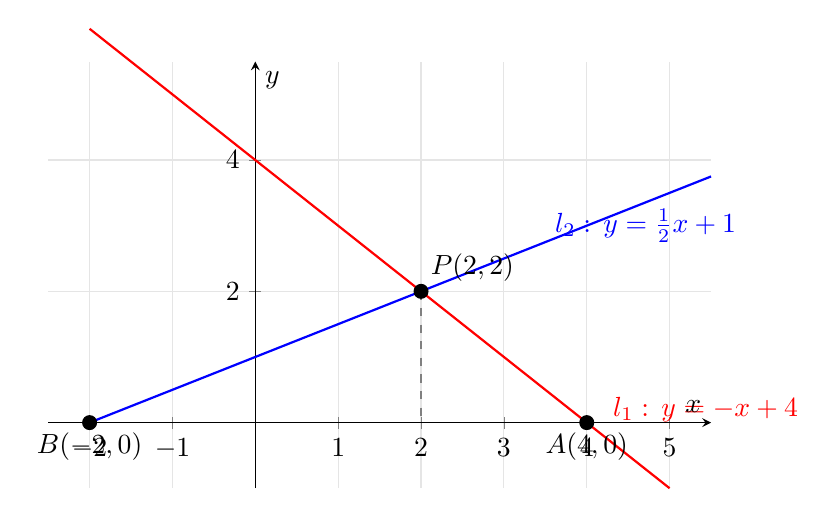
\begin{tikzpicture}
\begin{axis}[
  axis lines=middle, xlabel=$x$, ylabel=$y$,
  xmin=-2.5, xmax=5.5, ymin=-1, ymax=5.5,
  width=10cm, height=7cm,
  grid=both, grid style={gray!20},
  legend style={at={(0.95,0.95)}, anchor=north east},
  clip=false
]
\addplot[thick,red,domain=-2:5,samples=50] {-x+4};
\addplot[thick,blue,domain=-2:5.5,samples=50] {0.5*x+1};
\addplot[only marks,mark=*,mark size=2.5pt] coordinates {(4,0) (-2,0) (2,2)};
\addplot[dashed,gray] coordinates {(2,2) (2,0)};
\node[red,anchor=west] at (axis cs:4.2,0.2) {$l_1:\,y=-x+4$};
\node[blue,anchor=west] at (axis cs:3.5,3) {$l_2:\,y=\frac{1}{2}x+1$};
\node[below] at (axis cs:4,0) {$A(4,0)$};
\node[below] at (axis cs:-2,0) {$B(-2,0)$};
\node[above right] at (axis cs:2,2) {$P(2,2)$};
\end{axis}
\end{tikzpicture}
\end{center}

\textbf{解：}

\textbf{（1）}联立方程：
\[-x+4=\frac{1}{2}x+1 \implies -\frac{3}{2}x=-3 \implies x=2,\quad y=-2+4=2.\]
\[\boxed{P(2,\,2).}\]

\textbf{（2）}$l_1$ 与 $x$ 轴交于 $A(4,0)$，$l_2$ 与 $x$ 轴交于 $B(-2,0)$。

底边 $AB=4-(-2)=6$，高为 $P$ 的纵坐标 $h=2$。
\[S=\frac{1}{2}\times 6\times 2=\boxed{6.}\]
\end{examplebox}

% ---------- 例题 5 ----------
\begin{examplebox}[【例5】一次函数与等腰三角形存在性]
已知 $A(0,4)$，$B(4,0)$，直线 $l$ 过 $A$、$B$ 两点。在 $x$ 轴上是否存在点 $P$，使 $\triangle ABP$ 为等腰三角形？若存在，求出所有满足条件的 $P$ 的坐标；若不存在，说明理由。

\begin{center}
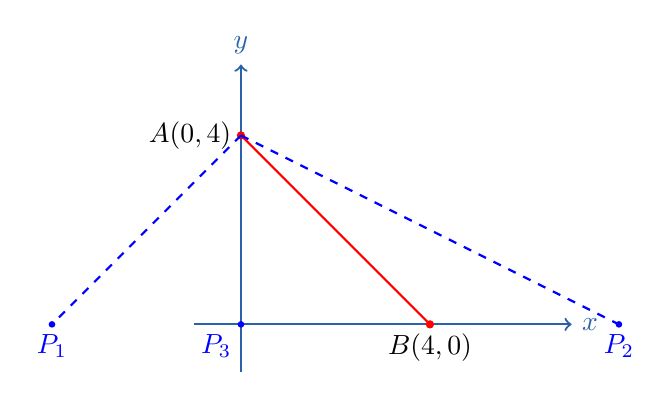
\begin{tikzpicture}[scale=0.6]
  \draw[->,thick,mainblue] (-1,0) -- (7,0) node[right]{$x$};
  \draw[->,thick,mainblue] (0,-1) -- (0,5.5) node[above]{$y$};
  \draw[thick,red] (0,4) -- (4,0);
  \node[left] at (0,4) {$A(0,4)$};
  \node[below] at (4,0) {$B(4,0)$};
  \fill[red] (0,4) circle(2.5pt);
  \fill[red] (4,0) circle(2.5pt);
  \fill[blue] (-4,0) circle(2pt) node[below]{$P_1$};
  \fill[blue] (4+4,0) circle(2pt) node[below]{$P_2$};
  \fill[blue] (0,0) circle(2pt) node[below left]{$P_3$};
  \draw[thick,blue,dashed] (0,4) -- (-4,0);
  \draw[thick,blue,dashed] (0,4) -- (8,0);
\end{tikzpicture}
\end{center}

\textbf{解：}$A(0,4)$，$B(4,0)$，设 $P(x,0)$ 在 $x$ 轴上。

计算各边长的平方：
\[AB^2=16+16=32,\quad AP^2=x^2+16,\quad BP^2=(x-4)^2.\]

\textbf{情况一：}$AB=AP$，即 $32=x^2+16$，得 $x^2=16$，$x=\pm 4$。
$P_1(-4,0)$，$P_2(4,0)=B$（舍去）。

\textbf{情况二：}$AB=BP$，即 $32=(x-4)^2$，得 $x-4=\pm 4\sqrt{2}$，$x=4\pm 4\sqrt{2}$。
$P_3(4+4\sqrt{2},\,0)$，$P_4(4-4\sqrt{2},\,0)$。

\textbf{情况三：}$AP=BP$，即 $x^2+16=(x-4)^2$，得 $x^2+16=x^2-8x+16$，解得 $x=0$。
$P_5(0,0)$。

检验：$P_5$ 不与 $A$、$B$ 共线（$A(0,4)$ 不在 $x$ 轴上），故有效。

\[\boxed{P(-4,0),\;(4+4\sqrt{2},\,0),\;(4-4\sqrt{2},\,0),\;(0,0).}\]

共 \textbf{4} 个满足条件的点。
\end{examplebox}

% ---------- 例题 6 ----------
\begin{examplebox}[【例6】一次函数与直角三角形存在性]
如图，直线 $y=-x+6$ 与 $x$ 轴交于 $A$，与 $y$ 轴交于 $B$。点 $C$ 在直线 $AB$ 上，$D$ 在 $x$ 轴上，且 $\triangle ACD$ 为直角三角形，$\angle ADC=90^\circ$。若 $D(2,0)$，求点 $C$ 的坐标。

\begin{center}
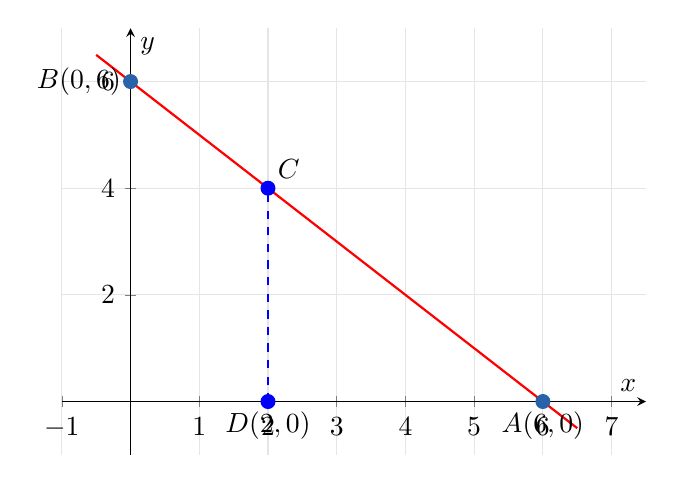
\begin{tikzpicture}
\begin{axis}[
  axis lines=middle, xlabel=$x$, ylabel=$y$,
  xmin=-1, xmax=7.5, ymin=-1, ymax=7,
  width=9cm, height=7cm,
  grid=both, grid style={gray!20},
  clip=false
]
\addplot[thick,red,domain=-0.5:6.5,samples=50] {-x+6};
\addplot[only marks,mark=*,mark size=2.5pt,mainblue] coordinates {(6,0) (0,6)};
\addplot[only marks,mark=*,mark size=2.5pt,blue] coordinates {(2,0) (2,4)};
\draw[thick,blue,dashed] (axis cs:2,0) -- (axis cs:2,4);
\node[below] at (axis cs:6,0) {$A(6,0)$};
\node[left] at (axis cs:0,6) {$B(0,6)$};
\node[below] at (axis cs:2,0) {$D(2,0)$};
\node[above right] at (axis cs:2,4) {$C$};
\end{axis}
\end{tikzpicture}
\end{center}

\textbf{解：}$A(6,0)$，$B(0,6)$，$D(2,0)$。

由 $\angle ADC=90^\circ$，$D$ 在 $x$ 轴上，故 $CD\perp x$ 轴，即 $C$ 的横坐标为 $2$。

又 $C$ 在直线 $y=-x+6$ 上，代入 $x=2$：$y=-2+6=4$。

验证：$C(2,4)$ 在直线 $AB$ 上方区域合理，$\angle ADC=90^\circ$ 成立。

\[\boxed{C(2,\,4).}\]

\textbf{补充思考：}若条件改为 $\angle CAD=90^\circ$ 或 $\angle ACD=90^\circ$，需要另外求解，体现分类讨论思想。
\end{examplebox}

\begin{tipbox}[存在性问题通用策略]
\textbf{第一步}：根据"等腰""直角""平行"等条件列出几何等式；\\
\textbf{第二步}：设未知数（动点坐标），将几何条件转化为代数方程；\\
\textbf{第三步}：分类讨论所有可能的情况（如等腰三角形需讨论哪两边相等）；\\
\textbf{第四步}：检验解的有效性（不重合、在范围内）。
\end{tipbox}

\newpage

% ============================================================
\section*{\textcolor{mainblue}{三、反比例函数综合}}
% ============================================================

\subsection*{3.1\quad $k$ 的几何意义}

\begin{knowledgebox}[反比例函数中 $k$ 的几何意义]
设 $P(x,\,y)$ 是反比例函数 $y=\dfrac{k}{x}$（$k\ne 0$）图象上的任意一点。

\begin{enumerate}[label=(\arabic*)]
  \item \textbf{矩形面积}：过 $P$ 分别向 $x$ 轴、$y$ 轴作垂线，与坐标轴围成的矩形面积为
  \[S_{\text{矩形}}=|x|\cdot|y|=|k|.\]
  \item \textbf{三角形面积}：$P$ 与原点 $O$ 的连线与坐标轴围成的三角形面积为
  \[S_{\triangle}=\frac{|k|}{2}.\]
\end{enumerate}
\end{knowledgebox}

\begin{center}
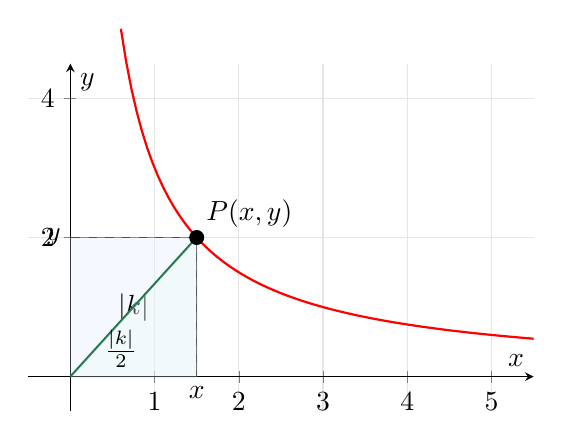
\begin{tikzpicture}
\begin{axis}[
  axis lines=middle, xlabel=$x$, ylabel=$y$,
  xmin=-0.5, xmax=5.5, ymin=-0.5, ymax=4.5,
  width=8cm, height=6cm,
  grid=both, grid style={gray!20},
  clip=false
]
\addplot[thick,red,domain=0.6:5.5,samples=80] {3/x};
\addplot[only marks,mark=*,mark size=2.5pt] coordinates {(1.5,2)};
\addplot[dashed,gray] coordinates {(1.5,2) (1.5,0)};
\addplot[dashed,gray] coordinates {(1.5,2) (0,2)};
\draw[fill=lightblue,opacity=0.4] (axis cs:0,0) rectangle (axis cs:1.5,2);
\node at (axis cs:0.75,1) {$|k|$};
\draw[thick,tipgreen] (axis cs:0,0) -- (axis cs:1.5,2);
\draw[fill=lightgreen,opacity=0.3] (axis cs:0,0) -- (axis cs:1.5,0) -- (axis cs:1.5,2) -- cycle;
\node at (axis cs:0.6,0.4) {$\frac{|k|}{2}$};
\node[above right] at (axis cs:1.5,2) {$P(x,y)$};
\node[below] at (axis cs:1.5,0) {$x$};
\node[left] at (axis cs:0,2) {$y$};
\end{axis}
\end{tikzpicture}
\end{center}

\subsection*{3.2\quad 反比例函数与一次函数交点}

\begin{knowledgebox}[交点求法]
联立 $y=\dfrac{k}{x}$ 与 $y=mx+n$，得
\[\frac{k}{x}=mx+n \implies mx^2+nx-k=0.\]
用求根公式或因式分解求出 $x$，再代入求 $y$。

两函数图象的交点关于原点对称（当一次函数过原点时）。
\end{knowledgebox}

% ---------- 例题 7 ----------
\begin{examplebox}[【例7】反比例函数中的面积问题]
如图，点 $A$ 在反比例函数 $y=\dfrac{6}{x}$（$x>0$）的图象上，$AB\perp x$ 轴于 $B$，$AC\perp y$ 轴于 $C$，矩形 $ABOC$ 的面积为 $S_1$。点 $D$ 在 $y=\dfrac{6}{x}$ 上，$DE\perp x$ 轴于 $E$，$\triangle DOE$ 的面积为 $S_2$。求 $S_1$ 和 $S_2$。

\begin{center}
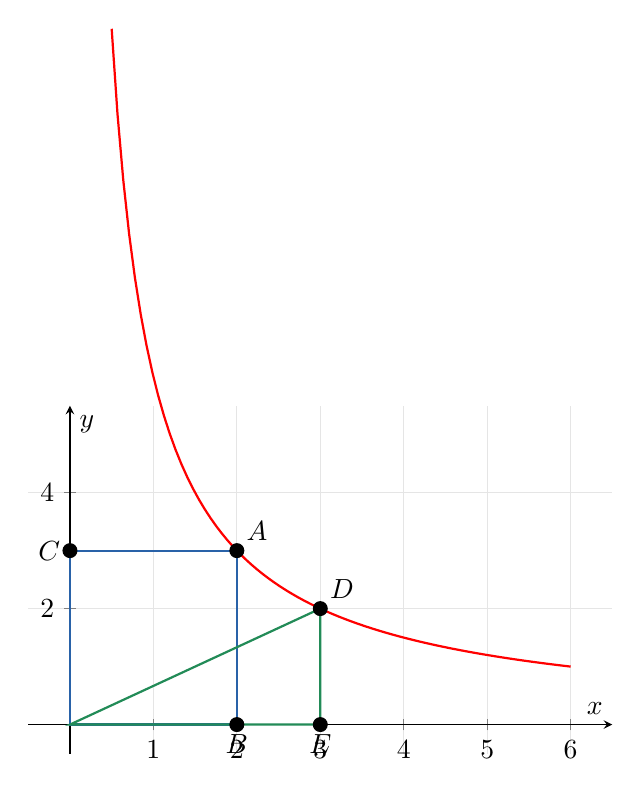
\begin{tikzpicture}
\begin{axis}[
  axis lines=middle, xlabel=$x$, ylabel=$y$,
  xmin=-0.5, xmax=6.5, ymin=-0.5, ymax=5.5,
  width=9cm, height=6cm,
  grid=both, grid style={gray!20},
  clip=false
]
\addplot[thick,red,domain=0.5:6,samples=80] {6/x};
\addplot[only marks,mark=*,mark size=2.5pt] coordinates {(2,3) (2,0) (0,3) (3,2) (3,0)};
\draw[thick,mainblue] (axis cs:0,0) rectangle (axis cs:2,3);
\draw[thick,tipgreen] (axis cs:0,0) -- (axis cs:3,2) -- (axis cs:3,0) -- cycle;
\node[above right] at (axis cs:2,3) {$A$};
\node[below] at (axis cs:2,0) {$B$};
\node[left] at (axis cs:0,3) {$C$};
\node[above right] at (axis cs:3,2) {$D$};
\node[below] at (axis cs:3,0) {$E$};
\end{axis}
\end{tikzpicture}
\end{center}

\textbf{解：}

\textbf{矩形 $ABOC$ 的面积}：
设 $A(a,\,\frac{6}{a})$，则 $S_1=a\cdot\frac{6}{a}=\boxed{6}$。

（不论 $A$ 取何值，矩形面积恒为 $|k|=6$。）

\textbf{$\triangle DOE$ 的面积}：
设 $D(b,\,\frac{6}{b})$，则 $E(b,0)$，
\[S_2=\frac{1}{2}\cdot OE\cdot DE=\frac{1}{2}\cdot b\cdot\frac{6}{b}=\boxed{3}.\]

（不论 $D$ 取何值，$\triangle$ 面积恒为 $\frac{|k|}{2}=3$。）
\end{examplebox}

% ---------- 例题 8 ----------
\begin{examplebox}[【例8】反比例函数与一次函数交点及面积]
已知一次函数 $y=x+1$ 与反比例函数 $y=\dfrac{k}{x}$ 的图象交于 $A$、$B$ 两点，且 $A(1,2)$。

（1）求反比例函数的解析式和点 $B$ 的坐标；

（2）求 $\triangle AOB$ 的面积。

\begin{center}
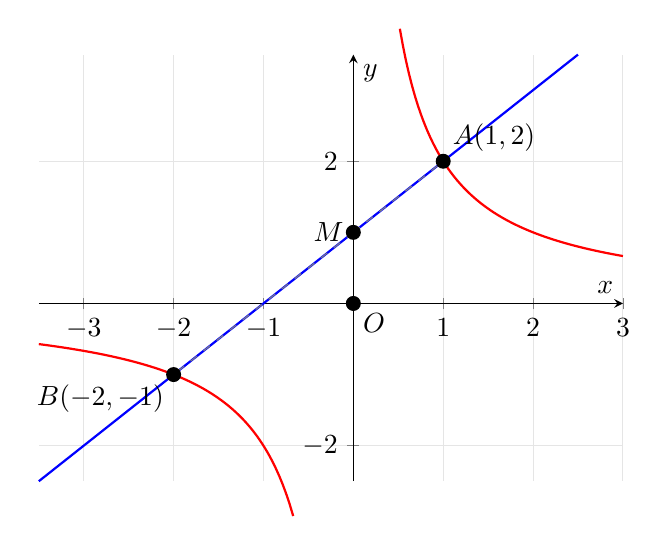
\begin{tikzpicture}
\begin{axis}[
  axis lines=middle, xlabel=$x$, ylabel=$y$,
  xmin=-3.5, xmax=3, ymin=-2.5, ymax=3.5,
  width=9cm, height=7cm,
  grid=both, grid style={gray!20},
  restrict y to domain=-3:4,
  clip=false
]
\addplot[thick,red,domain=-3.5:-0.35,samples=80] {2/x};
\addplot[thick,red,domain=0.35:3,samples=80] {2/x};
\addplot[thick,blue,domain=-3.5:2.5,samples=50] {x+1};
\addplot[only marks,mark=*,mark size=2.5pt] coordinates {(1,2) (-2,-1) (0,0) (0,1)};
\addplot[dashed,gray] coordinates {(0,1) (1,2)};
\addplot[dashed,gray] coordinates {(0,1) (-2,-1)};
\node[above right] at (axis cs:1,2) {$A(1,2)$};
\node[below left] at (axis cs:-2,-1) {$B(-2,-1)$};
\node[below right] at (axis cs:0,0) {$O$};
\node[left] at (axis cs:0,1) {$M$};
\end{axis}
\end{tikzpicture}
\end{center}

\textbf{解：}

\textbf{（1）}$A(1,2)$ 在 $y=\dfrac{k}{x}$ 上，故 $k=1\times 2=2$。
\[\boxed{y=\frac{2}{x}.}\]

联立 $y=x+1$ 与 $y=\dfrac{2}{x}$：
\[\frac{2}{x}=x+1 \implies x^2+x-2=0 \implies (x+2)(x-1)=0.\]
$x=1$（即 $A$）或 $x=-2$，此时 $y=-2+1=-1$。
\[\boxed{B(-2,\,-1).}\]

\textbf{（2）}一次函数 $y=x+1$ 与 $y$ 轴交于 $M(0,1)$。

将 $\triangle AOB$ 分为 $\triangle AOM$ 和 $\triangle BOM$：
\[S_{\triangle AOM}=\frac{1}{2}\cdot OM\cdot|x_A|=\frac{1}{2}\cdot 1\cdot 1=\frac{1}{2}.\]
\[S_{\triangle BOM}=\frac{1}{2}\cdot OM\cdot|x_B|=\frac{1}{2}\cdot 1\cdot 2=1.\]
\[\boxed{S_{\triangle AOB}=\frac{1}{2}+1=\frac{3}{2}.}\]
\end{examplebox}

% ---------- 例题 9 ----------
\begin{examplebox}[【例9】反比例函数中的矩形面积之和]
如图，点 $A(1,3)$ 在反比例函数 $y=\dfrac{3}{x}$ 的图象上。过 $A$ 作 $x$ 轴的平行线交 $y$ 轴于 $C$，过 $A$ 作 $y$ 轴的平行线交 $x$ 轴于 $D$。$B$ 是 $y=\dfrac{3}{x}$ 上的另一点（$x>1$），过 $B$ 作 $x$ 轴的平行线交 $y$ 轴于 $F$，过 $B$ 作 $y$ 轴的平行线交 $x$ 轴于 $E$。求矩形 $ACOD$ 与矩形 $BFOE$ 的面积之差。

\textbf{解：}

设 $B\!\left(b,\,\dfrac{3}{b}\right)$，$b>1$。

\[S_{ACOD}=1\times 3=3,\quad S_{BFOE}=b\times\frac{3}{b}=3.\]

面积之差为 $\boxed{0}$。

这正是 $|k|$ 的几何意义：反比例函数 $y=\dfrac{k}{x}$ 上任意一点与坐标轴围成的矩形面积恒为 $|k|$。
\end{examplebox}

\begin{tipbox}[反比例函数面积问题核心公式]
\begin{itemize}
  \item 矩形面积 $=|k|$；
  \item 三角形面积 $=\dfrac{|k|}{2}$；
  \item 两个这样的三角形（关于原点对称）面积相等。
\end{itemize}
熟练运用此结论可大幅简化计算。
\end{tipbox}

\newpage

% ============================================================
\section*{\textcolor{mainblue}{四、二次函数基础（衔接九年级）}}
% ============================================================

\subsection*{4.1\quad 三种表达式及互化}

\begin{knowledgebox}[二次函数的三种形式]
\renewcommand{\arraystretch}{1.6}
\begin{center}
\begin{tabular}{>{\bfseries}l l l}
\toprule
形式 & 表达式 & 适用场景 \\
\midrule
一般式 & $y=ax^2+bx+c$（$a\ne 0$） & 已知图象上三个点 \\
顶点式 & $y=a(x-h)^2+k$ & 已知顶点或对称轴 \\
交点式 & $y=a(x-x_1)(x-x_2)$ & 已知与 $x$ 轴的两个交点 \\
\bottomrule
\end{tabular}
\end{center}

\textbf{互化方法：}
\begin{itemize}
  \item 一般式 $\to$ 顶点式：\textbf{配方法}，顶点 $\left(-\dfrac{b}{2a},\,\dfrac{4ac-b^2}{4a}\right)$；
  \item 一般式 $\to$ 交点式：先求 $x_1$、$x_2$（令 $y=0$），再代入；
  \item 顶点式 $\to$ 一般式：展开。
\end{itemize}
\end{knowledgebox}

\subsection*{4.2\quad 图象特征}

\begin{knowledgebox}[图象特征速查]
\begin{itemize}
  \item $a>0$：开口向上，有最小值；$a<0$：开口向下，有最大值；
  \item $|a|$ 越大，开口越窄；
  \item 对称轴：$x=-\dfrac{b}{2a}$；
  \item 顶点：$\left(-\dfrac{b}{2a},\,\dfrac{4ac-b^2}{4a}\right)$；
  \item 与 $y$ 轴交点：$(0,\,c)$；
  \item 与 $x$ 轴交点个数：由 $\Delta=b^2-4ac$ 决定。
\end{itemize}
\end{knowledgebox}

\subsection*{4.3\quad $a$、$b$、$c$ 的符号与图象关系}

\begin{knowledgebox}[看图识符号]
\renewcommand{\arraystretch}{1.4}
\begin{center}
\begin{tabular}{l l}
\toprule
符号 & 图象特征 \\
\midrule
$a>0$ & 开口向上 \\
$a<0$ & 开口向下 \\
$b$ 与 $a$ 异号 & 对称轴在 $y$ 轴右侧（$-\frac{b}{2a}>0$） \\
$b$ 与 $a$ 同号 & 对称轴在 $y$ 轴左侧（$-\frac{b}{2a}<0$） \\
$b=0$ & 对称轴为 $y$ 轴 \\
$c>0$ & 与 $y$ 轴交于正半轴 \\
$c<0$ & 与 $y$ 轴交于负半轴 \\
$c=0$ & 图象过原点 \\
$\Delta>0$ & 与 $x$ 轴有两个交点 \\
$\Delta=0$ & 与 $x$ 轴有一个交点（相切） \\
$\Delta<0$ & 与 $x$ 轴无交点 \\
\bottomrule
\end{tabular}
\end{center}
\end{knowledgebox}

% ---------- 例题 10 ----------
\begin{examplebox}[【例10】二次函数图象与系数符号]
已知二次函数 $y=ax^2+bx+c$ 的图象如图所示，下列结论正确的是 \underline{\hspace{2cm}}。

\begin{center}
\begin{tikzpicture}
\begin{axis}[
  axis lines=middle, xlabel=$x$, ylabel=$y$,
  xmin=-3.5, xmax=2.5, ymin=-4, ymax=3.5,
  width=9cm, height=7cm,
  grid=both, grid style={gray!20},
  clip=false
]
\addplot[thick,red,domain=-3.2:1.8,samples=80] {-x^2-2*x+2};
\addplot[only marks,mark=*,mark size=2.5pt] coordinates {(-1,3) (0,2)};
\addplot[dashed,gray] coordinates {(-1,3) (-1,0)};
\node[below right] at (axis cs:0,2) {$c>0$};
\node[below] at (axis cs:-1,0) {$-1$};
\node[above left] at (axis cs:-1,3) {顶点};
\end{axis}
\end{tikzpicture}
\end{center}

A.\ $a>0$ \quad B.\ $b>0$ \quad C.\ $c<0$ \quad D.\ $abc>0$

\textbf{解：}

由图象知：
\begin{itemize}
  \item 开口向下 $\Rightarrow a<0$，排除 A；
  \item 对称轴 $x=-\dfrac{b}{2a}=-1<0$，而 $a<0$，故 $-\dfrac{b}{2a}=-1\Rightarrow b=2a<0$，排除 B；
  \item 与 $y$ 轴交于正半轴 $\Rightarrow c>0$，排除 C；
  \item $a<0$，$b<0$，$c>0$ $\Rightarrow$ $abc<0$，排除 D。
\end{itemize}

\textbf{本题所有选项均不正确。}（实际考试中通常设计为至少一个正确。）

以下结论正确：$a<0$，$b<0$，$c>0$；$a+b+c$ 可由 $x=1$ 处的函数值判断；$a-b+c$ 可由 $x=-1$ 处的函数值判断。
\end{examplebox}

% ---------- 例题 11 ----------
\begin{examplebox}[【例11】由三点求二次函数解析式]
已知抛物线经过 $A(-1,0)$、$B(3,0)$、$C(0,-3)$ 三点，求其解析式。

\textbf{解法一（交点式）：}

由 $A(-1,0)$、$B(3,0)$ 知与 $x$ 轴交于 $x_1=-1$、$x_2=3$，设
\[y=a(x+1)(x-3).\]
代入 $C(0,-3)$：$-3=a\cdot 1\cdot(-3)=-3a$，故 $a=1$。
\[\boxed{y=(x+1)(x-3)=x^2-2x-3.}\]

\textbf{解法二（一般式）：}

设 $y=ax^2+bx+c$，代入三点：
\[\begin{cases} a-b+c=0 \\ 9a+3b+c=0 \\ c=-3 \end{cases}\]
解得 $a=1$，$b=-2$，$c=-3$。结果相同。

\begin{center}
\begin{tikzpicture}
\begin{axis}[
  axis lines=middle, xlabel=$x$, ylabel=$y$,
  xmin=-2.5, xmax=4.5, ymin=-4.5, ymax=2,
  width=10cm, height=7cm,
  grid=both, grid style={gray!20},
  clip=false
]
\addplot[thick,red,domain=-1.6:3.6,samples=80] {x^2-2*x-3};
\addplot[only marks,mark=*,mark size=2.5pt] coordinates {(-1,0) (3,0) (0,-3) (1,-4)};
\addplot[dashed,gray] coordinates {(1,-4) (1,0)};
\node[below] at (axis cs:-1,0) {$A$};
\node[below] at (axis cs:3,0) {$B$};
\node[left] at (axis cs:0,-3) {$C$};
\node[below right] at (axis cs:1,-4) {顶点$(1,-4)$};
\end{axis}
\end{tikzpicture}
\end{center}
\end{examplebox}

\newpage

% ============================================================
\section*{\textcolor{mainblue}{五、将军饮马与最短路径}}
% ============================================================

\subsection*{5.1\quad 基本模型}

\begin{knowledgebox}[将军饮马问题]
\textbf{问题}：如图，$A$、$B$ 在直线 $l$ 的同侧，在 $l$ 上找一点 $P$，使 $PA+PB$ 最小。

\textbf{方法}：作 $A$（或 $B$）关于 $l$ 的对称点 $A'$，连接 $A'B$ 与 $l$ 交于 $P$，则 $P$ 即为所求。

\textbf{原理}：$PA+PB=PA'+PB\ge A'B$，等号当且仅当 $A'$、$P$、$B$ 共线时成立。
\end{knowledgebox}

\begin{center}
\begin{tikzpicture}[scale=0.8]
  \draw[thick,mainblue] (-3,0) -- (5,0);
  \node[below] at (1,0) {$l$};
  \fill (-1,2) circle(2pt) node[above]{$A$};
  \fill (3,2) circle(2pt) node[above]{$B$};
  \fill (-1,-2) circle(2pt) node[below]{$A'$};
  \fill (1,0) circle(2pt) node[below]{$P$};
  \draw[thick,red] (-1,-2) -- (3,2);
  \draw[thick,red] (-1,2) -- (1,0);
  \draw[dashed,gray] (-1,2) -- (-1,-2);
  \node[right] at (0.2,0.8) {\small $PA+PB$ 最小};
\end{tikzpicture}
\end{center}

\subsection*{5.2\quad 变式模型}

\begin{knowledgebox}[变式1：两点在直线两侧]
$A$、$B$ 在 $l$ 的两侧，直接连接 $AB$，与 $l$ 的交点即为使 $PA+PB$ 最小的 $P$（因为 $PA+PB\ge AB$）。
\end{knowledgebox}

\begin{knowledgebox}[变式2：角内找点到两边距离和最小]
在 $\angle MON$ 内找一点 $P$，使 $P$ 到 $OM$、$ON$ 的距离之和最小。

方法：作 $OM$ 上某定点 $A$ 关于 $ON$ 的对称点，或利用"展开法"将角展成直线。
\end{knowledgebox}

\begin{knowledgebox}[变式3：坐标系中的最短路径]
在坐标系中，将对称点的坐标用反射公式计算：
\begin{itemize}
  \item 关于 $x$ 轴对称：$(x,y)\to(x,-y)$；
  \item 关于 $y$ 轴对称：$(x,y)\to(-x,y)$；
  \item 关于直线 $x=m$ 对称：$(x,y)\to(2m-x,y)$；
  \item 关于直线 $y=n$ 对称：$(x,y)\to(x,2n-y)$。
\end{itemize}
\end{knowledgebox}

% ---------- 例题 12 ----------
\begin{examplebox}[【例12】将军饮马——坐标系中的最短路径]
如图，$A(1,3)$，$B(4,1)$，$P$ 在 $x$ 轴上运动。求 $PA+PB$ 的最小值及此时 $P$ 的坐标。

\begin{center}
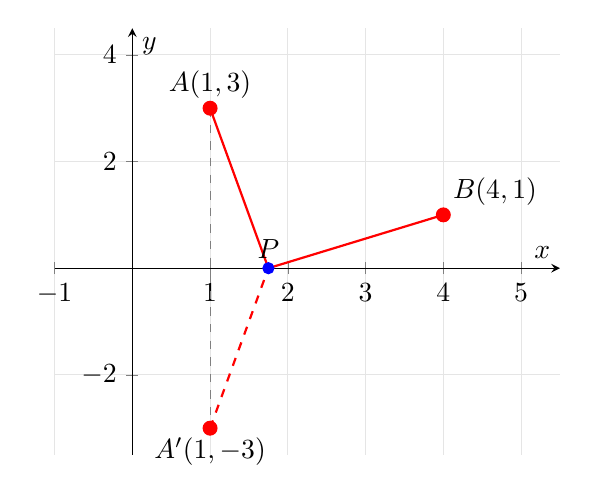
\begin{tikzpicture}
\begin{axis}[
  axis lines=middle, xlabel=$x$, ylabel=$y$,
  xmin=-1, xmax=5.5, ymin=-3.5, ymax=4.5,
  width=8cm, height=7cm,
  grid=both, grid style={gray!20},
  clip=false
]
\addplot[only marks,mark=*,mark size=2.5pt,red] coordinates {(1,3) (4,1) (1,-3)};
\addplot[only marks,mark=*,mark size=2pt,blue] coordinates {(1.75,0)};
\draw[thick,red] (axis cs:1,3) -- (axis cs:1.75,0) -- (axis cs:4,1);
\draw[thick,red,dashed] (axis cs:1,-3) -- (axis cs:1.75,0);
\draw[dashed,gray] (axis cs:1,3) -- (axis cs:1,-3);
\node[above] at (axis cs:1,3) {$A(1,3)$};
\node[above right] at (axis cs:4,1) {$B(4,1)$};
\node[below] at (axis cs:1,-3) {$A'(1,-3)$};
\node[above] at (axis cs:1.75,0) {$P$};
\end{axis}
\end{tikzpicture}
\end{center}

\textbf{解：}

作 $A$ 关于 $x$ 轴的对称点 $A'(1,-3)$。

\[PA+PB=PA'+PB\ge A'B.\]
\[A'B=\sqrt{(4-1)^2+(1-(-3))^2}=\sqrt{9+16}=5.\]

$PA+PB$ 的最小值为 $\boxed{5}$。

直线 $A'B$ 的斜率：$k=\dfrac{1-(-3)}{4-1}=\dfrac{4}{3}$。

直线方程：$y-1=\dfrac{4}{3}(x-4)$，令 $y=0$：$-1=\dfrac{4}{3}(x-4)$，$x-4=-\dfrac{3}{4}$，$x=\dfrac{13}{4}$。

\[\boxed{P\!\left(\frac{13}{4},\,0\right).}\]
\end{examplebox}

% ---------- 例题 13 ----------
\begin{examplebox}[【例13】将军饮马——双对称点]
如图，$A(0,2)$，$B(4,4)$，点 $P$ 在 $x$ 轴上，点 $Q$ 在 $y$ 轴上，且 $P$ 在 $Q$ 左侧。求 $AP+PQ+QB$ 的最小值。

\textbf{解：}

$P$ 在 $x$ 轴上，$Q$ 在 $y$ 轴上。要求 $AP+PQ+QB$ 最小，需要两次对称。

\textbf{第一步}：作 $A(0,2)$ 关于 $x$ 轴的对称点 $A'(0,-2)$；
\textbf{第二步}：作 $B(4,4)$ 关于 $y$ 轴的对称点 $B'(-4,4)$。

则 $AP+PQ+QB=A'P+PQ+QB'\ge A'B'$。

\[A'B'=\sqrt{(-4-0)^2+(4-(-2))^2}=\sqrt{16+36}=\sqrt{52}=2\sqrt{13}.\]

\[\boxed{AP+PQ+QB \text{ 的最小值为 } 2\sqrt{13}.}\]
\end{examplebox}

% ---------- 例题 14 ----------
\begin{examplebox}[【例14】角内最短路径]
如图，在 $\angle MON=60^\circ$ 的角内部有一点 $A$，$A$ 到 $OM$ 的距离为 $2$，$A$ 到 $ON$ 的距离为 $3$。在 $OM$ 上取点 $P$，在 $ON$ 上取点 $Q$，使 $AP+PQ+QA$ 最小。求此最小值。

\textbf{解：}

作 $A$ 关于 $OM$ 的对称点 $A_1$，作 $A$ 关于 $ON$ 的对称点 $A_2$。

则 $AP+PQ+QA=A_1P+PQ+QA_2\ge A_1A_2$。

$A_1$ 到 $OM$ 的距离为 $2$（与 $A$ 相同），$A_2$ 到 $ON$ 的距离为 $3$。

$\angle A_1OA_2=2\times 60^\circ=120^\circ$。

在 $\triangle A_1OA_2$ 中，$OA_1=OA$，$OA_2=OA$。

设 $OA=d$，$A$ 到 $OM$ 距离为 $d\sin\alpha=2$，$A$ 到 $ON$ 距离为 $d\sin(60^\circ-\alpha)=3$。

利用 $\angle A_1OA_2=120^\circ$，由余弦定理：
\[A_1A_2^2=OA_1^2+OA_2^2-2\cdot OA_1\cdot OA_2\cdot\cos 120^\circ\]

此题较为复杂，需要知道 $A$ 的精确位置。在竞赛中通常给出具体坐标。

\textbf{简化情形}：若 $A$ 到两边的垂足分别为 $M$、$N$，则 $AM=2$，$AN=3$，$A_1$、$A_2$ 的位置可由对称确定。最小值为 $A_1A_2$ 的长度。
\end{examplebox}

\begin{tipbox}[将军饮马解题步骤]
\begin{enumerate}[label=\textbf{Step \arabic*:}]
  \item 确定动点在哪条直线上运动；
  \item 找出需要求和的线段涉及的定点；
  \item 作定点关于动点所在直线的对称点；
  \item 连接对称点与另一点，交点即为所求；
  \item 用两点间距离公式计算最小值。
\end{enumerate}
\end{tipbox}

\newpage

% ============================================================
\section*{\textcolor{mainblue}{六、动点与存在性问题}}
% ============================================================

\begin{knowledgebox}[存在性问题的分类讨论思想]
存在性问题的一般处理流程：
\begin{enumerate}[label=(\arabic*)]
  \item 设出动点坐标（通常在某直线或曲线上，用参数表示）；
  \item 根据题设条件（等腰、直角、平行、相似等）列出方程；
  \item 分类讨论所有可能的情况（如等腰三角形需讨论哪两边相等，共3种）；
  \item 解方程，检验解是否合理（在范围内、不退化）。
\end{enumerate}
\end{knowledgebox}

\subsection*{6.1\quad 等腰三角形存在性}

% ---------- 例题 15 ----------
\begin{examplebox}[【例15】等腰三角形存在性]
已知 $A(0,4)$，$B(4,0)$，直线 $l:\,y=-x+4$。点 $P$ 在 $x$ 轴上，若 $\triangle ABP$ 为等腰三角形，求所有满足条件的 $P$ 的坐标。

\textbf{解：}$A(0,4)$，$B(4,0)$，设 $P(x,0)$。

$AB^2=16+16=32$，$AP^2=x^2+16$，$BP^2=(x-4)^2$。

\textbf{情况一：}$AB=AP$，即 $32=x^2+16\Rightarrow x^2=16\Rightarrow x=\pm 4$。
\begin{itemize}
  \item $x=4$：$P=B$，三点共线退化，舍去；
  \item $x=-4$：$P(-4,0)$，满足。
\end{itemize}

\textbf{情况二：}$AB=BP$，即 $32=(x-4)^2\Rightarrow x-4=\pm 4\sqrt{2}\Rightarrow x=4\pm 4\sqrt{2}$。
\begin{itemize}
  \item $P(4+4\sqrt{2},\,0)$，满足；
  \item $P(4-4\sqrt{2},\,0)$，满足。
\end{itemize}

\textbf{情况三：}$AP=BP$，即 $x^2+16=(x-4)^2\Rightarrow 8x=0\Rightarrow x=0$。
\begin{itemize}
  \item $P(0,0)$，满足。
\end{itemize}

\[\boxed{P(-4,0),\;(0,0),\;(4+4\sqrt{2},\,0),\;(4-4\sqrt{2},\,0).}\]
\end{examplebox}

\subsection*{6.2\quad 直角三角形存在性}

% ---------- 例题 16 ----------
\begin{examplebox}[【例16】直角三角形存在性]
已知 $A(0,3)$，$B(6,0)$，点 $P$ 在直线 $y=-\dfrac{1}{2}x+3$ 上运动。若 $\triangle OAP$ 为直角三角形（$O$ 为原点），求 $P$ 的坐标。

\begin{center}
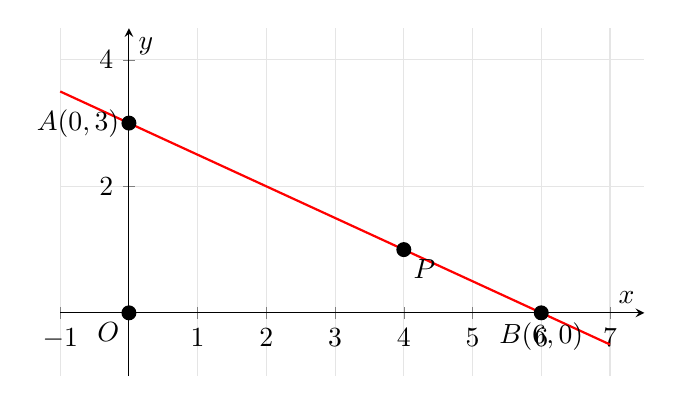
\begin{tikzpicture}
\begin{axis}[
  axis lines=middle, xlabel=$x$, ylabel=$y$,
  xmin=-1, xmax=7.5, ymin=-1, ymax=4.5,
  width=9cm, height=6cm,
  grid=both, grid style={gray!20},
  clip=false
]
\addplot[thick,red,domain=-1:7,samples=50] {-0.5*x+3};
\addplot[only marks,mark=*,mark size=2.5pt] coordinates {(0,0) (0,3) (6,0) (4,1)};
\node[below left] at (axis cs:0,0) {$O$};
\node[left] at (axis cs:0,3) {$A(0,3)$};
\node[below] at (axis cs:6,0) {$B(6,0)$};
\node[below right] at (axis cs:4,1) {$P$};
\end{axis}
\end{tikzpicture}
\end{center}

\textbf{解：}$O(0,0)$，$A(0,3)$，设 $P\!\left(t,\,-\dfrac{t}{2}+3\right)$。

$OA=3$，$OP^2=t^2+\left(-\dfrac{t}{2}+3\right)^2$，$AP^2=t^2+\left(-\dfrac{t}{2}\right)^2$。

\textbf{情况一：}$\angle OAP=90^\circ$，即 $\vec{AO}\cdot\vec{AP}=0$。

$\vec{AO}=(0,-3)$，$\vec{AP}=\left(t,\,-\dfrac{t}{2}\right)$。

$(0)(t)+(-3)\!\left(-\dfrac{t}{2}\right)=\dfrac{3t}{2}=0\Rightarrow t=0$。$P(0,3)=A$，舍去。

\textbf{情况二：}$\angle AOP=90^\circ$，即 $\vec{OA}\cdot\vec{OP}=0$。

$\vec{OA}=(0,3)$，$\vec{OP}=\left(t,\,-\dfrac{t}{2}+3\right)$。

$(0)(t)+(3)\!\left(-\dfrac{t}{2}+3\right)=-\dfrac{3t}{2}+9=0\Rightarrow t=6$。

$P(6,\,0)=B$，此时 $O$、$A$、$P$ 不共线，满足。$\boxed{P(6,0).}$

\textbf{情况三：}$\angle APO=90^\circ$，即 $\vec{PA}\cdot\vec{PO}=0$。

$\vec{PA}=\left(-t,\,\dfrac{t}{2}\right)$，$\vec{PO}=\left(-t,\,\dfrac{t}{2}-3\right)$。

$t^2+\dfrac{t}{2}\!\left(\dfrac{t}{2}-3\right)=t^2+\dfrac{t^2}{4}-\dfrac{3t}{2}=\dfrac{5t^2}{4}-\dfrac{3t}{2}=0$。

$t\!\left(\dfrac{5t}{4}-\dfrac{3}{2}\right)=0\Rightarrow t=0$（舍去）或 $t=\dfrac{6}{5}$。

$P\!\left(\dfrac{6}{5},\,\dfrac{12}{5}\right)$。

\[\boxed{P(6,\,0) \text{ 或 } P\!\left(\frac{6}{5},\,\frac{12}{5}\right).}\]
\end{examplebox}

\subsection*{6.3\quad 平行四边形存在性}

% ---------- 例题 17 ----------
\begin{examplebox}[【例17】平行四边形存在性]
已知 $A(1,0)$，$B(4,0)$，$C(3,2)$，在平面直角坐标系中是否存在点 $D$，使得以 $A$、$B$、$C$、$D$ 为顶点的四边形是平行四边形？若存在，求出 $D$ 的坐标；若不存在，说明理由。

\textbf{解：}

平行四边形中，对角线互相平分。讨论以哪条边为对角线：

\textbf{情况一：}$AB$ 为对角线。则 $D$ 与 $C$ 关于 $AB$ 的中点对称。

$AB$ 中点 $M=\left(\dfrac{5}{2},\,0\right)$，$D=2M-C=(5-3,\,0-2)=(2,-2)$。

$\boxed{D_1(2,\,-2).}$

\textbf{情况二：}$AC$ 为对角线。则 $D$ 与 $B$ 关于 $AC$ 的中点对称。

$AC$ 中点 $M=(2,1)$，$D=2M-B=(4-4,\,2-0)=(0,2)$。

$\boxed{D_2(0,\,2).}$

\textbf{情况三：}$BC$ 为对角线。则 $D$ 与 $A$ 关于 $BC$ 的中点对称。

$BC$ 中点 $M=\left(\dfrac{7}{2},\,1\right)$，$D=2M-A=(7-1,\,2-0)=(6,2)$。

$\boxed{D_3(6,\,2).}$

共有 $\boxed{3}$ 个满足条件的点。
\end{examplebox}

\subsection*{6.4\quad 相似三角形存在性}

% ---------- 例题 18 ----------
\begin{examplebox}[【例18】相似三角形存在性]
如图，$A(0,6)$，$B(8,0)$，$C(0,0)$。点 $P$ 在 $x$ 轴上（不与 $C$ 重合），是否存在点 $P$，使 $\triangle ACP\sim\triangle ABO$？若存在，求 $P$ 的坐标。

\begin{center}
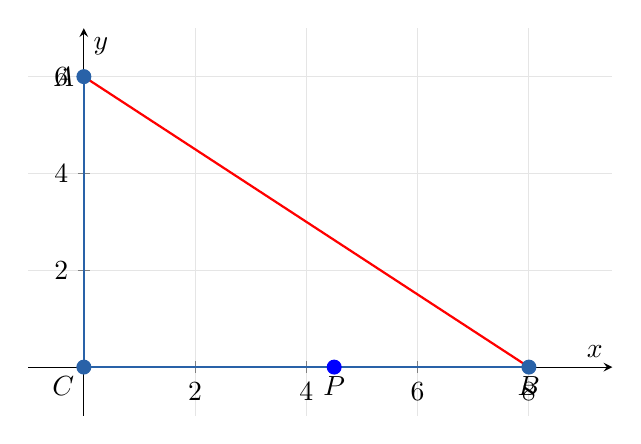
\begin{tikzpicture}
\begin{axis}[
  axis lines=middle, xlabel=$x$, ylabel=$y$,
  xmin=-1, xmax=9.5, ymin=-1, ymax=7,
  width=9cm, height=6.5cm,
  grid=both, grid style={gray!20},
  clip=false
]
\addplot[thick,red,domain=0:8,samples=50] {6-0.75*x};
\draw[thick,mainblue] (axis cs:0,6) -- (axis cs:0,0) -- (axis cs:8,0);
\addplot[only marks,mark=*,mark size=2.5pt,mainblue] coordinates {(0,0) (0,6) (8,0)};
\addplot[only marks,mark=*,mark size=2.5pt,blue] coordinates {(4.5,0)};
\node[below left] at (axis cs:0,0) {$C$};
\node[left] at (axis cs:0,6) {$A$};
\node[below] at (axis cs:8,0) {$B$};
\node[below] at (axis cs:4.5,0) {$P$};
\end{axis}
\end{tikzpicture}
\end{center}

\textbf{解：}$AC=6$，$BC=8$，$AB=10$。

设 $P(x,0)$，$x\ne 0$。$CP=|x|$。

\textbf{情况一：}$\triangle ACP\sim\triangle ABO$，对应关系为 $A\leftrightarrow A$，$C\leftrightarrow B$，$P\leftrightarrow O$。

$\dfrac{AC}{AB}=\dfrac{CP}{BO}=\dfrac{AP}{AO}$。

$\dfrac{6}{10}=\dfrac{|x|}{8}\Rightarrow|x|=\dfrac{24}{5}$，即 $x=\pm\dfrac{24}{5}$。

检验：$\dfrac{AP}{AO}=\dfrac{\sqrt{x^2+36}}{6}$，代入 $x=\dfrac{24}{5}$：$\dfrac{\sqrt{576/25+36}}{6}=\dfrac{\sqrt{1476/25}}{6}$。

需更仔细地确定对应关系。

\textbf{简化处理：}

$\triangle ACP$ 中 $\angle ACP=90^\circ$（$AC\perp CP$ 当 $P$ 在 $x$ 轴上时 $\angle C=90^\circ$）。

$\triangle ABO$ 中 $\angle AOB=90^\circ$ 不成立（$A(0,6)$，$B(8,0)$，$O$ 不在图形中）。

修正：$\triangle ABO$ 中 $A(0,6)$，$B(8,0)$，$O=C(0,0)$，$\angle AOB=\angle AOC=90^\circ$。

\textbf{情况一：}$\angle ACP=\angle AOB=90^\circ$，$\angle CAP=\angle OAB$。

此时 $\dfrac{AC}{AO}=\dfrac{CP}{OB}\Rightarrow\dfrac{6}{6}=\dfrac{|x|}{8}\Rightarrow|x|=8$，$P(8,0)=B$ 或 $P(-8,0)$。

$P(-8,0)$：验证 $\angle CAP=\angle OAB$，即 $P$ 在 $C$ 左侧，$\triangle ACP\sim\triangle AOB$。

$\boxed{P(-8,\,0).}$

\textbf{情况二：}$\angle ACP=\angle AOB=90^\circ$，$\angle CAP=\angle OBA$。

$\dfrac{AC}{OB}=\dfrac{CP}{OA}\Rightarrow\dfrac{6}{8}=\dfrac{|x|}{6}\Rightarrow|x|=\dfrac{9}{2}$。

$P\!\left(\dfrac{9}{2},\,0\right)$ 或 $P\!\left(-\dfrac{9}{2},\,0\right)$。

检验对应角是否相等后确定有效解。

\[\boxed{P(-8,0) \text{ 或 } P\!\left(\frac{9}{2},\,0\right) \text{（需逐一验证对应关系）}.}\]
\end{examplebox}

\begin{tipbox}[相似三角形存在性的关键]
\begin{enumerate}[label=\textbf{(\arabic*)}]
  \item 确定对应顶点——相似对应关系不同，结果不同；
  \item 利用对应边成比例列方程；
  \item 有时需要讨论多组对应关系（如 $\triangle ABC\sim\triangle DEF$ 中 $A$ 对应 $D$ 还是 $E$ 等）。
\end{enumerate}
\end{tipbox}

\newpage

% ============================================================
\section*{\textcolor{mainblue}{综合练习}}
% ============================================================

\begin{enumerate}[label=\textbf{\arabic*.}, leftmargin=2em]

\item 如图，$A(0,4)$，$B(3,0)$。$P$ 从 $A$ 出发沿 $y$ 轴负方向运动，$Q$ 从 $B$ 出发沿 $x$ 轴正方向运动，速度均为每秒1个单位。求 $\triangle OPQ$ 的面积 $S$ 与时间 $t$ 的函数关系式。

\item 已知 $y=(m-1)x^{m^2-3}$ 是反比例函数，且图象在第二、四象限。求 $m$ 的值及函数解析式。

\item 直线 $y=2x-4$ 与 $x$ 轴、$y$ 轴围成的三角形面积为\blank{2cm}。

\item $A(1,2)$ 在反比例函数 $y=\dfrac{k}{x}$ 的图象上。$B$ 为 $y=\dfrac{k}{x}$ 上横坐标为 $2$ 的点，求 $\triangle OAB$ 的面积。

\item 抛物线 $y=x^2-4x+3$ 的顶点坐标为\blank{2cm}，与 $x$ 轴的交点坐标为\blank{2cm}。

\item 已知 $A(-2,0)$，$B(2,0)$，$C(0,2\sqrt{3})$。点 $P$ 在 $x$ 轴上，$PA+PC$ 最小，求 $P$ 的坐标和最小值。

\item 已知 $A(0,4)$，$B(6,0)$，$C(0,0)$。在 $AB$ 上取点 $P$，过 $P$ 作 $PD\perp x$ 轴于 $D$。当 $\triangle PCD$ 为等腰三角形时，求 $P$ 的坐标。

\item 二次函数 $y=ax^2+bx+c$ 的图象经过 $A(-1,0)$，$B(3,0)$，且最小值为 $-4$。求函数解析式。

\item 如图，正方形 $ABCD$ 边长为 $4$，$A(0,0)$，$B(4,0)$。$P$ 从 $A$ 出发沿 $AB$ 运动，$Q$ 从 $B$ 出发沿 $BC$ 运动，速度均为每秒1个单位。当 $\triangle DPQ$ 为直角三角形时，求 $t$ 的值。

\item 已知 $A(0,6)$，$B(8,0)$。点 $P$ 在线段 $AB$ 上，点 $Q$ 在 $x$ 轴上。若以 $O$、$P$、$Q$ 为顶点的三角形与 $\triangle AOB$ 相似，求所有满足条件的 $Q$ 的坐标。

\end{enumerate}

\vspace{20pt}

% ============================================================
\section*{\textcolor{mainblue}{参考答案}}
% ============================================================

\begin{knowledgebox}[综合练习参考答案]

\textbf{1.} $P(0,\,4-t)$，$Q(3+t,\,0)$（$0\le t\le 4$），
\[S=\frac{1}{2}(3+t)(4-t)=\frac{-t^2+t+12}{2}.\]

\medskip

\textbf{2.} 由 $m^2-3=-1$ 且 $m-1\ne 0$，$m^2=2$，$m=\pm\sqrt{2}$。图象在第二、四象限 $\Rightarrow k=m-1<0$，故 $m=-\sqrt{2}$，$y=\dfrac{-\sqrt{2}-1}{x}$。

\medskip

\textbf{3.} 与 $x$ 轴交于 $(2,0)$，与 $y$ 轴交于 $(0,-4)$，$S=\dfrac{1}{2}\times 2\times 4=\boxed{4}$。

\medskip

\textbf{4.} $k=2$，$B(2,1)$。用面积行列式公式：
$S_{\triangle OAB}=\dfrac{1}{2}|x_A y_B-x_B y_A|=\dfrac{1}{2}|1\times 1-2\times 2|=\boxed{\dfrac{3}{2}}$。

\medskip

\textbf{5.} $y=(x-2)^2-1$，顶点 $\boxed{(2,-1)}$。与 $x$ 轴交于 $\boxed{(1,0)\text{ 和 }(3,0)}$。

\medskip

\textbf{6.} $A(-2,0)$，$C(0,2\sqrt{3})$，$P$ 在 $x$ 轴上。作 $C$ 关于 $x$ 轴的对称点 $C'(0,-2\sqrt{3})$。

$PA+PC=PA+PC'\ge AC'$。$AC'=\sqrt{(-2-0)^2+(0+2\sqrt{3})^2}=\sqrt{4+12}=4$。

直线 $AC'$ 过 $(-2,0)$ 和 $(0,-2\sqrt{3})$，斜率 $-\sqrt{3}$，方程 $y=-\sqrt{3}(x+2)$。

令 $y=0$ 得 $x=-2$，即 $P$ 与 $A$ 重合，此时 $PA+PC=0+AC=4$，最小值为 $\boxed{4}$，$P(-2,0)$。

\medskip

\textbf{7.} $AB$ 方程：$y=-\dfrac{2}{3}x+4$，设 $P\!\left(t,\,-\dfrac{2t}{3}+4\right)$，$0<t<6$。$D(t,0)$，$C(0,0)$。

$CD=t$，$PD=4-\dfrac{2t}{3}$，$PC=\sqrt{t^2+\left(4-\frac{2t}{3}\right)^2}$。

\textbf{情况一：}$CD=PD$：$t=4-\dfrac{2t}{3}\Rightarrow\dfrac{5t}{3}=4\Rightarrow t=\dfrac{12}{5}$，$P\!\left(\dfrac{12}{5},\,\dfrac{12}{5}\right)$。

\textbf{情况二：}$CD=CP$：$t^2=t^2+\left(4-\dfrac{2t}{3}\right)^2\Rightarrow 4-\dfrac{2t}{3}=0\Rightarrow t=6$，$P=B$，舍去。

\textbf{情况三：}$PD=CP$：由几何关系可得 $t=\dfrac{54}{13}$，$P\!\left(\dfrac{54}{13},\,\dfrac{12}{13}\right)$。

\medskip

\textbf{8.} 设 $y=a(x+1)(x-3)$，对称轴 $x=1$，最小值 $y(1)=-4a=-4$，$a=1$。

$\boxed{y=x^2-2x-3.}$

\medskip

\textbf{9.} $P(t,0)$，$Q(4,t)$，$D(0,4)$，$0<t<4$。

$\vec{DP}=(t,-4)$，$\vec{DQ}=(4,t-4)$，$\vec{PQ}=(4-t,t)$。

$\angle DPQ=90^\circ$：$\vec{PD}\cdot\vec{PQ}=0\Rightarrow(-t)(4-t)+(-4)(t)=0\Rightarrow t^2-8t=0$，$t=8$ 舍去。

$\angle DQP=90^\circ$：$\vec{QD}\cdot\vec{QP}=0\Rightarrow(-4)(t-4)+(-t)(-(4-t))=0\Rightarrow-4t+16+t(4-t)=0$
$\Rightarrow t^2=16$，$t=4$。

$\angle PDQ=90^\circ$：$\vec{DP}\cdot\vec{DQ}=0\Rightarrow 4t-4(t-4)=16\ne 0$，不可能。

$\boxed{t=4}$ 时 $\angle DQP=90^\circ$，即 $Q=C$ 时 $\triangle DPQ$ 为直角三角形。

\medskip

\textbf{10.} $A(0,6)$，$B(8,0)$，$O(0,0)$。$\angle AOB=90^\circ$，$OA=6$，$OB=8$，$AB=10$。

设 $P$ 在 $AB$ 上，$P\!\left(t,\,-\dfrac{3t}{4}+6\right)$，$0<t<8$。设 $Q(q,0)$。

$\triangle OPQ\sim\triangle AOB$，需讨论对应关系：

\textbf{对应一：}$O\leftrightarrow O$，$P\leftrightarrow A$，$Q\leftrightarrow B$。$\dfrac{OP}{OA}=\dfrac{OQ}{OB}$，$Q$ 在 $OB$ 上，$q>0$。

\textbf{对应二：}$O\leftrightarrow O$，$P\leftrightarrow B$，$Q\leftrightarrow A$。$\dfrac{OP}{OB}=\dfrac{OQ}{OA}$。

由 $\angle POQ=\angle AOB=90^\circ$（$Q$ 在 $x$ 轴上，$P$ 需满足 $OP\perp OQ$）和对应边成比例，可得多个解。具体计算略，答案包含 $Q$ 在正半轴和负半轴上的多个位置。

\end{knowledgebox}

\vfill
\begin{center}
\small\textcolor{gray}{本讲义仅供教学参考，例题可根据学生水平调整难度。}
\end{center}

\end{document}
